\chapter{\DS Equations}
\label{chap:DSE}

\section{Quark DSE}
The \DS equations (DSE) are the analogue of Euler-Lagrange equations for the quantum field theory, since they are the equations of motion of the corresponding Green's function. Here we are only interested in the derivation of the quark \DS equations, though the same ideas can be applied for gluons and ghosts as well, for a more detailed derivation, see \cite{Roberts:1994dr}. At first, we focus on single color quark field $q(x)$, since quark colors enter in QCD Lagrangian as a cumulative sum. Also we drop a ghost fields from considering, since they are not coupled directly to the quarks, but only through the full gluon propagator and quark-gluon vertex and hence do not enter to quark DSE explicitly.  \\

The starting point of the derivation is that, the functional integral of a total functional derivative is zero given the fields vanish at a boundary:
%
\beqa
	\int \mathcal{D}q\frac{\delta}{\delta q}  = 0\;.
\eeqa
%
We employ this observation in order to derive the quark DSE, by taking the functional derivative of generating functional of QCD in respect to quark field $\bar{q}$: 
%
\beqa
\label{dse:tot_deriv}
\notag	0 &=& \int \mathcal{D} [A \bar q q] \frac{\delta}{\delta \bar{q}} \; \text{exp}  \left\lbrace i \int d^4x \left( \mathcal{L}_{QCD} + J^{a\mu} A^a_\mu + \bar q \eta + \bar \eta q \right)  \right\rbrace \;,\; \\
	&=& \left[ \frac{\delta S_{QCD}}{\delta \bar{q}} \left( -i\frac{\delta}{\delta J}, -i\frac{\delta}{\delta \bar{\eta}}, i\frac{\delta}{\delta \eta} \right) + \eta(x) \right]  \mathcal{Z}[A \bar \eta \eta] \;,
\eeqa
%
where $S_{QCD}=\int d^4x \mathcal{L}^{QCD}$ and $\mathcal{L}^{QCD}$ is given by \Eq{\ref{qcd_low:L_QCD}}. Further, following to Itzykson and Zuber \cite{itzykson2012quantum}, we rewrite $\mathcal{Z}[A \bar \eta \eta]$ in terms of generating functional of connected Green's functions, setting $\mathcal{Z}[A \bar \eta \eta] = \text{exp}(\mathcal{G}[A \bar \eta \eta])$. By that we introduce the generating functional for the connected, one-particle irreducible (1PI) correlation functions:
%
\beqa
	\mathcal{G}[A \bar q q] \equiv i\Gamma[q, \bar{q}, A^\mu] + i \int d^4x \left[ \bar{q}\eta + q\bar{\eta} + A_\mu J^\mu \right] 
\eeqa
%
After taking the derivative in \Eq{\ref{dse:tot_deriv}} and setting all sources to zero $\eta = \bar{\eta} = J = 0$ we obtain:
%
\beqa
\label{dse:DSE_coord}
%0 = \left[ \eta(x) + \left( i\dslash - m + g\gamma^\mu(-i)\frac{\delta}{\delta J^\mu(x)}(-i)\frac{\delta}{\delta \bar{\eta}(x)} \right)  \right] \mathcal{Z}[A \bar \eta \eta] \;. 
\notag &\delta^4(x-y) = (i\dslash - m)S(x-y) - \\
&-ig^2 \!\bigintsss\! d^4z_1 d^4z_2 d^4z_3 \gamma_\mu D^{\mu\nu}(x-z_1)S(x - z_2)\Gamma_\nu(z_2,z_3;z_1)S(z_3-y) \;,\;\;\;\;
\eeqa
%
where we identified corresponding functional derivatives of $\Gamma[q, \bar{q}, A^\mu]$ as following:
%
\beqa
	S(x-y) = \left(\left. \frac{\delta^2 \Gamma}{\delta \bar{q}(x) \delta q(y)}\right\vert_{\bar{q}=q=A^\mu=0} \right)^{-1}	\;, \\
	D^{\mu\nu}(x-y) = \left(\left. \frac{\delta^2 \Gamma}{\delta A^\mu(x) \delta A^\nu(y)}\right\vert_{\bar{q}=q=A^\mu=0} \right)^{-1}	\;, \\
	g \Gamma_\mu(x,y;z) = \left. \frac{\delta}{\delta A^\mu(z)}\frac{\delta^2 \Gamma}{\delta \bar{q}(x) \delta q(y)} \right\vert_{\bar{q}=q=A^\mu=0} \;.
\eeqa
which are the quark propagator $S(x-y)$, the gluon propagator $D^{\mu\nu}(x-y)$ and the quark-gluon vertex $\Gamma_\mu(x,y;z)$, that should not be confused with the generating functional $\Gamma[q, \bar{q}, A^\mu]$.  
\begin{figure*}[t]
\tiny
 \begin{center}
  \includegraphics[width=0.95\textwidth]{figures/quark_DSE_gen.png}
 \end{center}
 \caption{\footnotesize Quark \DS equations, circles denote dressed propagators and vertexes.}\label{fig:quark_DSE_gen} 
\end{figure*}
The \Eq{\ref{dse:DSE_coord}} is the quark propagator in coordinate space. Multiplying with $S^{-1}(y-y^{\prime})$ , integrating over $y^\prime$ and performing the standard Fourier transformation gives the quark DSE in momentum space:
\beqa
	\label{dse:DSE_mom}
	S^{-1}(p) = (i\pslash - m) - ig^2\int \frac{d^4k}{(2\pi)^4} D^{\mu\nu}(k)\gamma_\mu S(q) \Gamma_\nu(p,q)\;.
\eeqa
So far we considered a single color structure, which obviously does not represent a full picture of the underlying physics. Thus we need to introduce the color structure into \Eq{\ref{dse:DSE_mom}}, by interchanging $\Gamma_\nu(p,q) \rightarrow  \Gamma^a_\nu(p,q)$, where $a=1,...,8$ denotes an index in $SU(3)$ adjoint representation, and also $\gamma_\mu \rightarrow \lambda^a \gamma_\mu$, where $\lambda^a$ are Gellmann matrices. Additionally the quark propagators carry implicitly the color index $i=1,2,3$, being the fundamental object of $SU(3)$ color group. Applying the aforementioned changes, we obtain the proper quark \DS equations:
\beqa
\label{dse:DSE_mom_full}
	S^{-1}(p) = (i\pslash - m) - ig^2\int \frac{d^4k}{(2\pi)^4} D^{\mu\nu}(k) \delta^{ab} \lambda^a \gamma_\mu S(q) \Gamma^b_\nu(p,q)\;.
\eeqa
This is integral equation is represented diagrammatically on Fig. \ref{fig:quark_DSE_gen}.
The full gluon propagator $D^{\mu\nu}(k)$ and full quark-gluon vertex $\Gamma_\nu(p,q)$ in \Eq{\ref{dse:DSE_mom_full}} satisfy their own DSEs, which connect them to higher n-point Green functions and by that create an infinite tower of equations. \\

However, this not final point of the derivation, since we have not yet defined the renormalization properties of the involved objects. The parameters like gauge coupling and quark mass are not physical and therefore should be expressed through experimental quantities. We achieve this by the multiplicative renormalization, which leads to the following replacements:
\beqa
	\label{dse:renorm}
\notag	&g=Z_g \tilde{g}\;, \;\;\; m = Z_m \tilde{m}\;, \\
	&S(p) = Z_2 \tilde{S}(p)\;, \;\; D^{\mu\nu}(k) = Z_3 \tilde D^{\mu\nu}(k)\;, \;\; \Gamma_\nu(p,q) = Z^{-1}_{1F} \tilde \Gamma_\nu(p,q)\;. \;\; \;\;\;\;\;\;
\eeqa
Here the $Z_{g,m,2,3,1F}$ are the renormalization factors for corresponding objects and tilde sign denotes the renormalized quantity. Note that this factors can be related to each other by universality of gauge coupling for any interaction vertices and due Slavnov-Taylor identity \cite{0201524724}. The following relations read as:
\beqa
	\label{dse:renorm_relations}
	&Z_g^{-1} = Z_3^{1/2} Z_2 Z^{-1}_{1F} = Z_3^{3/2} Z_1^{-1} = Z_3 Z_4^{-1/2} = Z_3^{1/2} \tilde Z_3 \tilde Z_1^{-1}\;, \\
	&\frac{Z_3}{Z_1} = \frac{Z_2}{Z_{1F}} = \frac{Z_3^{1/2}}{Z_4^{1/2}} = \frac{\tilde{Z_3}}{\tilde{Z_1}}\;,
\eeqa
where $Z_1, Z_4, \tilde{Z_3}, \tilde{Z_1}$ are the renormalization factors of the 3-gluon vertex, the 4-gluon vertex, the ghost propagator and the ghost-gluon vertex correspondingly. Using the aforementioned relations we can finally derive quark \DS equations for renormalized objects: 
\beqa
	\label{dse:DSE_full_renorm}
	S^{-1}(p) = Z_2(i\dslash - m) - ig^2Z_{1F}\int \frac{d^4}{(2\pi)^4} D^{\mu\nu}(k) \delta^{ab} \lambda^a \gamma_\mu S(q) \Gamma^b_\nu(p,q)\;,\;\;
\eeqa
suppressing a tilde notation for the renormalized quantities. Since gluon and quark propagators in Minkowski space can expose a non-analytical behaviour, for a purpose of numerical calculations we perform the Wick rotation \cite{PhysRev.96.1124} and throughout this thesis consider all our equations to be in Euclidean space-time. The detailed instruction how the Wick rotation is done is given in Appendix \ref{app:euclidean} \\

The Eq.(\ref{dse:DSE_full_renorm}) contains important pieces, which have to be specified. $D^{\mu\nu}(k)$ is the dressed gluon propagator, that satisfies its own DSE and in Euclidean space and Landau gauge have the following general form:
\beqa
	D^{\mu\nu}(k) = \frac{G(k^2)}{k^2}\left( \delta^{\mu\nu} - \frac{k^\mu k^\nu}{k^2} \right) \;,
\eeqa 
where $G(k^2)$ is gluon dressing function, connected to the gluon vacuum polarisation function via $G(k^2)=1/(1 + \Pi(k^2))$. 
The dressed quark-gluon vertex $\Gamma_\nu(p,q)$ also posses its own DSE with the solution in its general form given by 12 scalar functions. The Dirac basis is generated by linear combination of three Lorenz vectors $\{ \gamma^\mu \;, p^\mu \;, q^\mu \}$, each multiplied with one of the four Lorenz scalar matrices $\{ \ONE\;, \pslash \;, \qslash \;, \sigma^{\mu\nu}p_\mu q_\nu\}$. This choice is not unique, the basis is constrained only by Lorentz transformation properties. The explicit expression of general quark-gluon vertex is given by:
\beqa
\label{dse:gluon_vertex_gen}
	\Gamma_\mu(p,q) = \sum_{i=1}^{12}V^i(p,q) T^i_\mu(p,q) \;,
\eeqa
where $T^i_\mu(p,q)$ is employed Dirac basis and $V^i(p,q)$ are scalar dressing functions of the quark-gluon vertex. \\

The general form of the solution for Eq. \ref{dse:DSE_full_renorm} is full (dressed) quark propagator, given in terms of two scalar dressing functions and corresponding Dirac basis and in Euclidean space can be written as:
\beqa
	\label{dse:S_gen}
	S^{-1}(p) = i\pslash A(p^2,\mu^2) + B(p^2,\mu^2) = Z^{-1}(p^2,\mu^2)[i\pslash + M(p^2)]\;,
\eeqa
where $Z(p^2,\mu^2)$ and $M(p^2)$ are the quark wave function renormalization and the dressed mass function respectively. At this point we explicitly declared the renormalization point $\mu$ dependence of the dressing functions and introduced the $\mu^2$ - the renormalization scale. In order to address the renormalization procedure we need to unfold Eq. \ref{dse:DSE_full_renorm} by projecting out equations for each dressing function $A(p^2)$ and $B(p^2)$, using projectors $P_A=-i\frac{\pslash}{p^2}$ and $P_B=\ONE$ correspondingly: 
\beqa
\label{dse:DSE_AB}
	A(p^2) &=& Z_2(\mu) + Z_{1F}C_Fg^2\int\frac{d^4}{(2\pi)^4} D^{\mu\nu}(k)\Tr\left[ P_A \gamma_\mu S(q) \Gamma^b_\nu(p,q) \right]\; \;\;\;\;\; \\
\notag	B(p^2) &=& m_R(\mu) + Z_{1F}C_Fg^2\int\frac{d^4}{(2\pi)^4} D^{\mu\nu}(k)\Tr\left[ P_B \gamma_\mu S(q) \Gamma^b_\nu(p,q) \right]\;, \;\;\;\;\;
\eeqa
here $C_F=4/3$ is the Casimir operator for color $SU(3)$ and the trace is performed over Dirac indexes. The renomalization constants $Z_2$ and $m_R$ can be obtained by applying the following renomalization conditions:
\beqa
	\label{dse:renorm_cons}
	A(\mu^2,\mu^2) &=& 1 \\
	B(\mu^2, \mu^2) &=& m_R \;,
\eeqa
after which the equations for constants $Z_2$ and $m_R$ read as:
\beqa
	Z_2(\mu^2,\Lambda^2) &=& 1 - A(\mu^2,\Lambda^2) \\
	m_R(\mu^2) &=& Z_2(\mu^2,\Lambda^2)m_{bare} - B(\mu^2,\Lambda^2) \;,
\eeqa
where $\Lambda^2$ is numerical integration cut-off. \\

The Eq. (\ref{dse:DSE_AB}) is a final representation of quark \DS equation, which is of immense importance, being the main piece of the whole framework. The quark DSE itself allows to study the chiral symmetry breaking and dynamical quark mass generation. It is the crucial building block for \BS equation and Faddeev equations - the two-body and three-body bound state equations correspondingly, which are to be considered in Chapter \ref{chap:BSE}. 


\section{Truncation}
\subsubsection*{Rainbow-ladder ansatz}
\label{sec:RL}
The essential input to quark DSE is full(dressed) gluon propagator and full(dressed) quark-gluon vertex, given by their own \DS equations, which are forming, as it was mentioned, an infinite tower of equations, setting relations between higher order n-point Green functions. Therefore in order to be able to solve them, we need to apply a certain truncation or \textit{ansatz} for these correlation functions. As a first step in this work we will consider a so-called \textit{rainbow-ladder} truncation \cite{Maris:1997hd}, that on quark DSE level leads to the replacement:
\beqa
	\label{dse:RL_trunc}
Z_{1F} \frac{g^2}{4\pi} D_{\mu\nu}(q)\Gamma^\nu(k,p) \rightarrow Z_2^2T_{\mu\nu}(q) 
\frac{\alpha_{\mathrm{eff}}(q^2)}{q^2}\gamma^\nu\;,
\eeqa
here the $T_{\mu\nu}(q)=\delta_{\mu \nu}-\frac{q_\mu q_\nu}{q^2}$ is the transverse projector and the $\alpha_{\mathrm{eff}}(q^2)$ is effective running coupling. This is the simplest \textit{ansatz} satisfying the axial Ward-Takahashi identity (axWTI), as we will discuss in Chapter \ref{chap:BSE}, and essentially takes into account only the $\gamma_\mu$-structure of the dressed quark-vertex and combines all dressing effects of the gluon and the vertex into an effective running coupling $\alpha_{\mathrm{eff}}(q^2)$ . The resulting diagram expression for quark \DS equations is given on Fig. \ref{fig:DSE_RL}.
\begin{figure}[H]
\tiny
 \begin{center}
  \includegraphics[width=0.95\textwidth]{figures/DSE_RL}
 \end{center}
 \caption{\footnotesize The quark \DS equations, within RL truncation. Lines with filled circles note fully dressed propagators.  }\label{fig:DSE_RL} 
\end{figure}
However, as we will show later, this truncation is very useful as a first exploratory step toward the reverse engineering of QCD at low energies. The resulting expression for the quark \DS equation reads as:
\beqa
\displaystyle S^{-1}(p)=Z_2 S^{-1}_0(p) + C_F (Z_2)^2 \int \frac{d^4 k}{(2\pi)^4} \gamma_{\mu} S(k) \gamma_{\nu} T_{\mu\nu}(q) \frac{4\pi\alpha_{\mathrm{eff}}(q^2)}{q^2}\;,
\label{dse:DSE_RL}
\eeqa
where $C_F=(N_c^2-1)/2N_c$ is the Casimir operator coming from the color trace. \\

The choice of $\alpha_{\mathrm{eff}}$ is dictated from one side by the phenomenologically
required infrared enhancement of the effective single gluon interaction, necessary for the dynamical 
generation of a constituent-like quark mass and a chiral vacuum quark condensate. From another side its ultraviolet behaviour has to match to the perturbative one and therefore ensure the preservation of one-loop results. As a model for $\alpha_{\mathrm{eff}}(q^2)$ that takes into account aforementioned criteria we take that of Maris and Tandy \cite{Maris:1999nt}, which explicit expression reads as following:
\beqa
\label{dse:MT_model}
\alpha_{\mathrm{eff}}(q^2)=\pi\eta^7x^2e^{-\eta^2x}
+\frac{2\pi\gamma_m\left(1-e^{-y}\right)}{\log\left[e^2-1+(1+z)^2\right]}\;,
\eeqa
where $x=q^2/\Lambda^2$, $y=q^2/\Lambda_t^2$, $z=q^2/\Lambda_{\mathrm{QCD}}^2$. 
Here $\Lambda_t=1$~GeV is a regularization parameter for the perturbative logarithm;
its value has no material impact on the numerical results. The QCD-scale 
$\Lambda_{\mathrm{QCD}}=0.234$~GeV controls the running of the logarithm with
anomalous dimension $\gamma_m=12/25$ corresponding to four active quark flavors.
The infrared strength of this model is controlled by the parameters $\Lambda$ and 
$\eta$. While $\Lambda = 0.72$ GeV is fixed from the pion decay constant, there is considerable
freedom to vary the dimensionless parameter $\eta$. The explicit view of this interaction model, with provided parameters, is given on Fig. \ref{fig:MT_graph}. 
\begin{figure*}[t]
\tiny
 \begin{center}
  \includegraphics[width=0.95\textwidth]{figures/Gluon_MT_graph}
 \end{center}
 \caption{\footnotesize Gluon dressing function $\frac{\alpha_{\mathrm{eff}}(q^2)}{q^2}$ in Maris--Tandy model \cite{Maris:1999nt}. The $\Lambda = 0.72$ GeV and $\eta = 1.8$ GeV }\label{fig:MT_graph} 
\end{figure*} \\

Despite the apparent simplicity of the gluon model and the truncation employed, this approach can successfully describe: light pseudoscalar and vector masses and decay constants\cite{Maris:1997tm, Maris:1999nt}, $\pi$, $K^+$, $K^0$ electromagnetic form factors\cite{Maris:2000sk}, $\gamma \pi \gamma$-transition\cite{Maris:2002mz}, strong decays\cite{Jarecke:2002xd}. In the course of this work the same approach with a few technical adjustments was used to describe the spectra of light and heavy mesons and to make a prediction for $J^{PC}=3^{--}$ for charmonium and bottomonium bound states \cite{Fischer:2014cfa, Fischer:2014xha}. This results are represented in Chapter \ref{chap:spectra}.
%
%
%
\subsubsection*{Unquenching effect}
However the \DS equations framework is not bounded to aforementioned truncation. Over the years were made a huge amount of successful efforts to go beyond Rainbow-Ladder approach. One of promising routes is to use explicit diagrammatic approximations to the DSE of the quark-gluon vertex \cite{Bender:1996bb,Watson:2004kd,Bhagwat:2004hn,Matevosyan:2006bk,Alkofer:2008tt,Fischer:2007ze,Fischer:2009jm}. 
\begin{figure}[H]
\tiny
 \begin{center}
  \includegraphics[width=0.95\textwidth]{figures/qqg_vertex_gen}
 \end{center}
 \caption{\footnotesize The full, untruncated \DSE for the quark-gluon vertex. }\label{fig:qqg_vertex_gen} 
\end{figure}
The the full, untruncated \DSE for the quark-gluon vertex is given diagrammatically in
Fig. \ref{fig:qqg_vertex_gen}. Here we are primarily interested in the mid-momentum behavior of the vertex and in particular in hadronic
contributions. To lowest order in a skeleton expansion such contributions can only occur in the diagram with the bare quark-gluon vertex at the external gluon line. 
\begin{figure}[H]
\tiny
 \begin{center}
  \includegraphics[width=0.95\textwidth]{figures/qqg_hadron}
 \end{center}
 \caption{\footnotesize The expansion in terms of hadronic and non-hadronic
contributions to the quark-antiquark scattering kernel. The dotted line describes mesons, the dashed line baryons and the double lines correspond to diquarks.  }\label{fig:qqg_hadron} 
\end{figure}
Consider this diagram that consists of quark-antiquark scattering kernel, which can be expanded in terms of one-particle irreducible Green's functions and resonance exchange contributions, as it is given on Fig. \ref{fig:qqg_hadron}. Of all those the term containing the pion one-meson exchange should be dominant, since further diagrams with exchange of heavy mesons and baryons, $(K, \rho, N, ...)$, are suppressed by their masses accordingly. 
This approximation allows to study the pion cloud effects on the spectrum of light mesons \cite{Fischer:2007ze,Fischer:2008sp,Fischer:2008wy} and 
baryons \cite{Sanchis-Alepuz:2014wea}. Also it is beneficial to have explicit hadronic degrees of freedom, since the pion cloud effects 
are expected to play an important role in the low momentum behaviour of form factors and hadronic decay processes of baryons
\cite{Thomas:1981vc,Miller:2002ig,Ramalho:2008dp,Cloet:2012cy,Eichmann:2011vu, Eichmann:2011aa,Sanchis-Alepuz:2013iia}. It should be noted, however, pions are not elementary fields and their wave functions must to be determined from their Bethe-Salpeter equation, as we will see in Chapter 4. \\

On another hand, the infrared domain of the quark propagator and its analytic structure heavily depends on the quark-gluon vertex truncations, such that, in principle all twelve Dirac structures from Eq. (\ref{dse:gluon_vertex_gen}) can be important \cite{Skullerud:2003qu,Kizilersu:2006et}. Therefore it is crucial to  utilise explicit notations for tensor structures of quark-gluon vertex beyond the leading $\gamma_\mu$ term \cite{Chang:2009zb,Chang:2010hb,Chang:2011ei,Heupel:2014ina,Williams:2014iea}. \\ 

In the course of this work we will incorporate into the coupled system of \DS and \BS equations the pion cloud effect, provided by scheme \cite{Fischer:2008wy}, where was obtained the good agreement with lattice QCD and meson phenomenology. Since this effect is generated due to the presence of dynamical sea quarks, it can be considered as unquenching effect. In this case the truncation take following form:
\beqa
	\label{dse:RL_pi_truncation}
Z_{1F} \frac{g^2}{4\pi} D_{\mu\nu}(q)\Gamma^\nu(k,p) \rightarrow Z_2^2T_{\mu\nu}(q) 
\frac{\alpha_{\mathrm{eff}}(q^2)}{q^2}\gamma^\nu -\frac{1}{C_F}\tau^iZ_2\gamma_5\Gamma_\pi ( \frac{p+k}{2};q )\;,
\eeqa
where $\tau^i$ are $SU(2)$ isospin symmetry generators and $\Gamma_\pi (\frac{p+k}{2};q)$ is the full pion wave function, evaluated at symmetrized momenta and given by 4 Dirac components:
\beqa
	\Gamma_\pi (p;P) = \gamma_5 \left[  E(p;P)\ONE + F(p;P)\Pslash + G(p;P)\pslash + H(p;P)\sigma^{\mu\nu}p_\mu P_\nu \right] 
	\label{dse:pion_vertex_gen}
\eeqa
On diagrammatical level this leads to addition of an extra diagram involving the pion exchange and pion wave function, as it is represented by Fig. \ref{fig:DSE_PS}.
\begin{figure}
\tiny
 \begin{center}
  \includegraphics[width=0.95\textwidth]{figures/DSE_with_pi}
 \end{center}
 \caption{\footnotesize The quark \DS equations, within Rainbow-Ladder truncation with unquenching pion cloud effect. Lines with filled circles note fully dressed propagators.  }\label{fig:DSE_PS} 
\end{figure}
The explicit form of corresponding quark DSE can be written as following:
\beqa
\displaystyle S^{-1}(p)=Z_2 S^{-1}_0(p) + C_F (Z_2)^2 \int \frac{d^4 k}{(2\pi)^4} \gamma_{\mu} S(k) \gamma_{\nu} T_{\mu\nu}(q) \frac{4\pi\alpha_{\mathrm{eff}}(q^2)}{q^2} \;\;\;\;\;\;\;\;\; \\
\notag - 3 \, Z_2 \int \frac{d^4 k}{(2\pi)^4} \left[\gamma_5 S(k) \Gamma_\pi ( \frac{p+k}{2};k-p ) + \gamma_5 S(k) \Gamma_\pi ( \frac{p+k}{2};p-k ) \right] \frac{D_\pi(q^2)}{2}
\label{dse:DSE_PS}
\eeqa
Where $q=p-k$, the quark renormalization constant $Z_2$, the fully dressed inverse quark propagator $S^{-1}(p)=i \slashed p A(p^2) + B(p^2)$, inverse bare one $S^{-1}_0(p)=i \slashed p  + m$ and $D_\pi(q^2)=\frac{1}{q^2+M^2_\pi}$.  
The first line is the Rainbow-Ladder contribution, where the same modelling was applied as in \ref{sec:RL}. The second line embodies the pion cloud effect, that satisfies the axial-vector Ward-Takahashi(AxWTI) identity, with the vertex $\Gamma_\pi (p;P)$ being the full pion wave function. Here, the coupling of the pion to the quark is given by a bare pseudoscalar vertex and a full pion Bethe-Salpeter amplitude. Note, however, that in general also the choice of two dressed vertices is possible and it is not clear a priori, which of the two choices is the better approximation of the original two-loop diagram. In \cite{Fischer:2008wy} the choice with one bare vertex led to satisfactory results in the vector-meson sector and we will therefore adopt this also here. \\

For a reasons of numerical simplicity we employ the approximation to the full pion Bethe-Salpeter wave function by the
leading amplitude $E(p;P)$ in the chiral limit, which is due to AxWTI given by \cite{Maris:1997hd}:
\beqa
	\Gamma_\pi(p;P) =\gamma_5 E(p;P) = \gamma_5 \frac{B(p^2)}{f_\pi}\;,
	\label{dse:pion_vertex}
\eeqa
where $B(p^2)$ is the scalar dressing function of the inverse quark propagator, taken in the chiral limit $m_q \rightarrow 0$. The $f_\pi = 93 \; \text{MeV}$ is the pion weak decay constant. This approximation omits the back-coupling effects of the three sub-leading amplitudes. Note however, this approximation is only strictly valid in chiral limit and approximately valid at physical pion mass point. For the high pion mass calculation carried out throughout this thesis we employed explicitly calculated first pion amplitude $E(p;P)$ in rainbow-ladder approach, continued into complex relative momentum $p$ via the same continuation procedure we used for the quark propagator, which is described in Appendix \ref{app:numerics}. As it was shown in Ref. \cite{Fischer:2008sp}, where full back-coupling has been evaluated in a real value approximation, the omission of $F(p;P), G(p;P), H(p;P)$ pion amplitudes leads to an error of only a few percent for meson masses and of about 10-20\% for decay constants for a physical pion. Note that we use aforementioned approximation only for the internal pion wave function, as it sets the interaction. The biggest advantage of the approximation Eq. (\ref{dse:pion_vertex}) compared to the full back-coupling performed in Ref. \cite{Fischer:2008sp} is that the Eq. (\ref{dse:DSE_PS}) can be solved self-consistently without any external input from pion \BS equation, so that it reduces the numerical efforts dramatically. \\

%
\section{Numerical solution of the DSE}
In this section we will demonstrate the numerical solutions of the Eq. \ref{dse:DSE_RL} and \ref{dse:DSE_PS}. Clearly the polarization tensor of the resulting dressed propagator must have the following form: $S(p) =i \sigma_v(p^2) \pslash + \sigma_s(p^2)$ and for inversed $S^{-1}(p)=-i A(p^2)\pslash + B(p^2)$, with $\sigma_v = \frac{A}{A^2 p^2 + B^2}$ and $\sigma_s = \frac{B}{A^2 p^2 + B^2}$. These unknown dressing functions $A(p^2)$ and $B(p^2)$ are the solution of quark \DS equations, which we intent to find. Throughout this work we apply the iteration method to solve the quark \DS equations, which appear to be nonlinear integral equations, and obtain aforementioned dressing functions. We put a more detailed description of this numerical procedure into Appendix \ref{app:numerics}. \\

At first we consider the Euclidean space solutions of quark DSE obtained within \textit{rainbow-ladder} truncation Eq. (\ref{dse:RL_trunc}), since the solving procedure does not require special treatment of the integration momenta as for the pion exchange. The resulting quark wave function $Z(p^2)$ and quark mass function $M(p^2)$ are shown on Fig. \ref{fig:quark_Z_func} and Fig. \ref{fig:quark_M_func} correspondingly. Note the gluon Maris-Tandy model parameters Eq. (\ref{dse:MT_model}) employed in this calculations are $\Lambda=0.72$ and $\eta=1.8$. The used renormalized current quark masses parameters for different flavor and type of quarks are of the same order as current quark masses in perturbative QCD and are given on Table. \ref{tab:mass_bare}. Note that we are consider the isosymmetric case, so the $m_{up}=m_{down}$.
\begin{table}[!h]
\renewcommand{\arraystretch}{1.3}
\begin{tabular*}{\columnwidth}{@{\extracolsep{\stretch{1}}}c|c|c|c|c|c@{}}
\hline
\hline
 & chiral & up/down & strange & charm & bottom \\
\hline
$m_{R} \; [GeV]$  & 0 & 0.0037 & 0.085 & 0.87 & 3.79 \\
\hline
\hline
\end{tabular*}
\caption{The values $m_{R}$ of used current quark mass parameters.  \label{tab:mass_bare}}
\end{table}
The renormalization point set to be $\mu=19\;\text{GeV}$. Aforementioned parameters are chosen to reproduce experimental masses of pion and rho mesons, $m_\pi, \; m_\rho$ and pion weak decay constant $f_\pi$, obtained via \BS equations as we will see in Chapter\;5 and are given in Table. \ref{tab:RL_params}.  \\
\begin{table*}
\centering
\renewcommand{\arraystretch}{1.3}
\begin{tabular}{c|c|c||c|}
\hline
\hline
          				     & \multicolumn{2}{c||}{RL1} & RL2 + pion cloud  \\
\hline
          				     & Light quark (u,d,s) & Heavy quarks (c,b) & Light quark (u,d,s) \\
 $\Lambda$ &  0.72    & 0.72 & 0.84 \\
$\eta$ & $1.8\pm 0.2$ & $1.257\pm 0.2$ & $1.8\pm 0.2$ \\                                                                                                                                                               
\hline
\hline
\end{tabular}
\caption{\footnotesize The values of effective single gluon model parameters.}\label{tab:RL_params}
\end{table*}
%
\begin{figure}
\tiny
 \begin{center}
  \includegraphics[width=0.95\textwidth]{figures/quark_Z_functions}
 \end{center}
 \caption{\footnotesize $Z(p^2)$ quark wave function renormalization for different types of quarks. The renormalizization point set to be $\mu=19\;\text{GeV}$. }\label{fig:quark_Z_func} 
\end{figure}

\begin{figure}
\tiny
 \begin{center}
  \includegraphics[width=0.95\textwidth]{figures/quark_M_functions}
 \end{center}
 \caption{\footnotesize $M(p^2)$ quark mass function for different types of quarks. The renormalizization point set to be $\mu=19\;\text{GeV}$. }\label{fig:quark_M_func} 
\end{figure}
The Fig. \ref{fig:quark_M_func} makes apparent that dynamical chiral symmetry (D$\chi$SB) is realized, i.e. in the rainbow-ladder truncation in a form Eq. (\ref{dse:RL_trunc}) with effective coupling given by Eq. (\ref{dse:MT_model}) the D$\chi$SB can provided. As we see in deep ultraviolet region the magnitude of $M(p^2)$ quark mass function is driven by renormalized quark mass, according to \cite{Miransky:1986ib}. It is logarithmicaly scaling down in a presence of explicit chiral breaking, i.e. non-zero bare quark mass $m_{bare}\neq 0$, as:
\beqa
	M(p^2) \approx \frac{1}{[\text{ln}(p^2/\Lambda^2_{QCD})]^{1/2\pi^2b}}
\eeqa
and in chiral case it is falling as $\mathbf{O}(1/p^2)$:
\beqa
	M(p^2) \approx \frac{1}{p^2}[\text{ln}(p^2/\Lambda^2_{QCD})]^{1/2\pi^2b-1}\;,
\eeqa
exposing irregular and regular behaviour respectively. In the infrared domain, however, the quark mass function enhances dramatically by orders of magnitude in comparison to current masses, especially for light quarks and chiral case. This enhancement is a clear evidence of dynamical mass generation from current quark mass to a constituent quark mass. Also this effect takes place at scale approximately $1\; \text{GeV}^2$, as it is meant to occur due to hadron phenomenology. Nevertheless, as will be shown in Chapter 5, the dynamically generated mass function in the chiral case used as input to pion \BS equations lead to zero pion mass $m_\pi=0$, fulfilling Gell-Mann--Oakes--Renner relation Eq. (\ref{qcd_low:GMOR}). \\ 
 \begin{figure*}[t]
 \begin{center}
  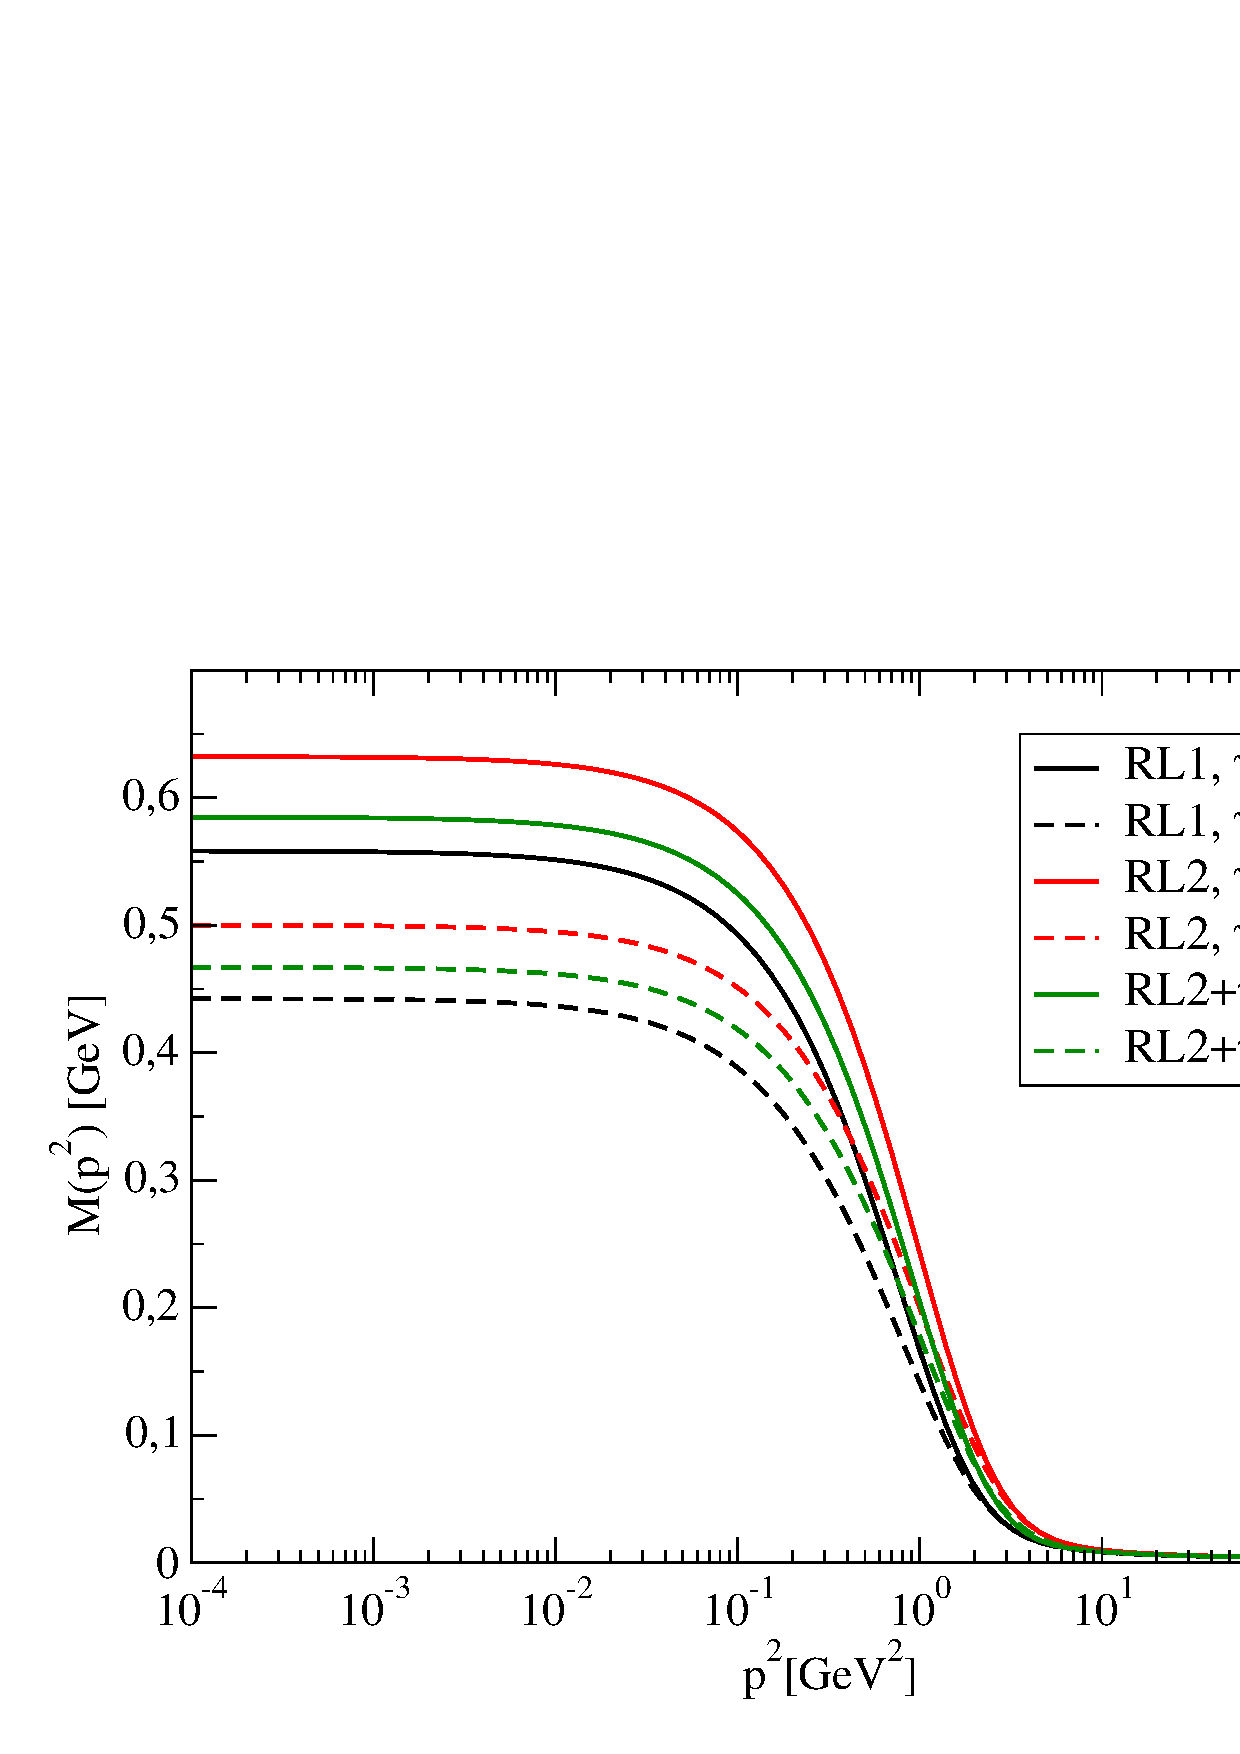
\includegraphics[width=0.95\textwidth,clip]{figures/mass}
 \end{center}
 \caption{$M(p^2)$ Quark mass function as function of the squared momentum.}\label{fig:RL_vs_PS}
\end{figure*}
In case of included pion cloud effect it requires extra numerical efforts to obtain the solutions. Similarly, the parameters $\Lambda$ and $\eta$ were fitted in order to reproduce experimental value of pion mass and pion decay constant, although the current mass of the up quark was kept the same. The new set of parameters are $\Lambda=0.84$ and $\eta=1.8$. The $\Lambda$ is increased to reflect the increased interaction range due to the added pion exchange. The resulting quark mass functions are displayed in Fig.~\ref{fig:RL_vs_PS}. For the 
two setups fixed by physical input, RL1 and RL2+$\pi$ given in Table \ref{tab:RL_params},
we find very similar mass functions with a difference in $M(0)$ of less than 
five percent. The quark-core setup $RL2$ generates slightly larger quark masses.
In general, the quark mass function encodes dynamical chiral symmetry breaking and 
nicely displays the transition from the low momentum notion of a constituent quark 
mass to the high momentum notion of a running current quark mass. Although the 
quark mass function is a renormalisation group invariant it is not, however, a 
gauge invariant quantity and therefore not directly observable. The chiral properties 
of our framework are also encoded in the dependence of the pion mass from the 
current quark mass. Further in Chapter \ref{chap:spectra} we explicitly checked the Gell-Mann-Oakes-Renner relation
for all setups and find that it holds within the numerical accuracy of 2 \%, 
as expected from the axWTI. 
\begin{figure}[h]
\tiny
 \begin{center}
  \includegraphics[width=0.95\textwidth]{figures/DSE_vs_Lattice}
 \end{center}
 \caption{\footnotesize The impact of pion cloud effect on $M(p^2)$ quark mass function.  }\label{fig:DSE_vs_Lattice} 
\end{figure}
	Also we compared our result to the lattice data on quenched and unquenched quark mass function in order to check the impact of unquenching effects, i.e. pion clouds with the lattice QCD. From the Fig. \ref{fig:DSE_vs_Lattice} we see that although the absolute value of $M(p^2)$ in infrared does not coincide with our calculations, the relative changes induced by unquenching pion cloud effect are of the similar size. It was shown in \cite{Fischer:2008sp}, that the usage of Ball-Chu vertex can provide a better agreement with lattice data. However, the inclusion of the pion exchange does not produce any qualitative difference in a behaviour of dressing functions, e.g. the most significant change happens in $M(p^2)$ quark mass function, where pion clouds lead to shrinking dynamical mass generation in infrared region by 10 percent. \\
		
Also it is important to consider the order parameter of dynamical chiral symmetry breaking - the quark condensate \cite{Miransky:271593}. Recall that in perturbative theory in chiral limit $m_q\rightarrow 0$ the dressing function $B(p^2)=0$ and therefore the mass function $M(p^2)=B(p^2)/A(p^2)=0$ as well. However as we see from Fig. \ref{fig:quark_M_func} the $M(P^2)$ is not zero in chiral limit. Thus, the quark condensate:
\beqa
	\langle \bar q q \rangle &=& - \lim_{\Lambda \rightarrow \inf} Z_4(\mu,\Lambda) \int^\Lambda \frac{d^4 k}{(2\pi)^4} \Tr \Bigl[ S_{m_bare = 0}(k) \Bigl] \\
	&=& - \lim_{\Lambda \rightarrow \inf} Z_4(\mu,\Lambda) \int^\Lambda \frac{d^4 k}{(2\pi)^4} \Tr \Bigl[ \frac{B(p^2)}{p^2A^2(p^2) + B^2(p^2)} \Bigl]\;,
\eeqa
is nonzero by virtue of a nonzero $B(p^2)$. Here $Z_4$ is quark mass renormalization constant, given by:
\beqa
	Z_4 = 2 - \frac{B(\mu^2,\Lambda^2)}{m_R(\mu^2)}
\eeqa
The resulting value for the quark condensate in rainbow-ladder and in pion cloud truncation are given in Table. \ref{tab:quark_cond}.
\begin{table}[!h]
\centering
\renewcommand{\arraystretch}{1.3}
\begin{tabular*}{0.70\textwidth}{@{\extracolsep{\stretch{1}}}c|c|c|c@{}}
\hline
\hline
 & RL1 & RL2 & RL2 + pion cloud \\
\hline
$\langle \bar q q\rangle \; [MeV]$  & 281 & 300 & 280 \\
\hline
\hline
\end{tabular*}
\caption{The values of the quark condencate for a rainbow-ladder and pion cloud truncation in comparisson.  \label{tab:quark_cond}}
\end{table}
 However, as we will see from Chapter\;4 the nonzero $B(p^2)$ in chiral case still generates the massless pion, thus ensuring the pions to be the Goldstone bosons. \\
%	
\subsection*{Continuation into time-like region}
The solutions of quark \DS equations we obtained so far are already a very valuable source of information about dynamical chiral symmetry breaking. However, as we stated earlier, the parameters of effective coupling should be fitted in a such way that the pion mass and weak decay constant are reproduced by \BS equation (BSE) of pion bound state. And this equations itself requires as input the solutions of the quark \DS equations (DSE). Due to certain kinematic scheme of BSE, which will be clarified in Chapter 5, the input from quark DSE must be provided partially in time-like region $p^2 < 0$. Namely on the contour in complex plane, which parametric form is defined by mass of bound state to be calculated:
\beqa
	p^2 = t^2 + itM_{state} - \frac{M_{state}^2}{4} 
	\label{dse:contour}
\eeqa
For the parameter $t \in [-\infty, \infty]$ defining the contour in complex plane, in our computations we use Legendre integration nodes. This specific form of the contour will be derived later, when the details of kinematic of the bound state BSE will be considered. \\
	
Brute-force way to the continuation is to invoke the Eq. (\ref{dse:DSE_RL}) on complex $p$-momentum, using space-like the solution $S(k)$ as input in equations. In this case the relative momenta $q=p-k$ will become complex as well and effective coupling model will be invoked in time-like region. There are several issues associated with the analytic continuation in this kinematic scheme: on one hand, the $q$-momentum is no longer real and therefore usage of Maris-Tandy(MT) model Eq. (\ref{dse:MT_model}) may produce numerical glitches; on another hand, in the pion propagator, given in form: $D_\pi(q^2)=\frac{1}{q^2+M^2_\pi}$, complex $q$-momenta will probe the pion pole, therefore diverging any integration. Thus this kinematic scheme can only be applied for Rainbow-ladder calculation. \\
	The resulting continuation in $\sigma_v = \frac{A}{A^2 p^2 + B^2}$ dressing function for quark propagator are given is Fig. \ref{fig:sigma_poles}. 
\begin{figure}
\tiny
 \begin{center}
  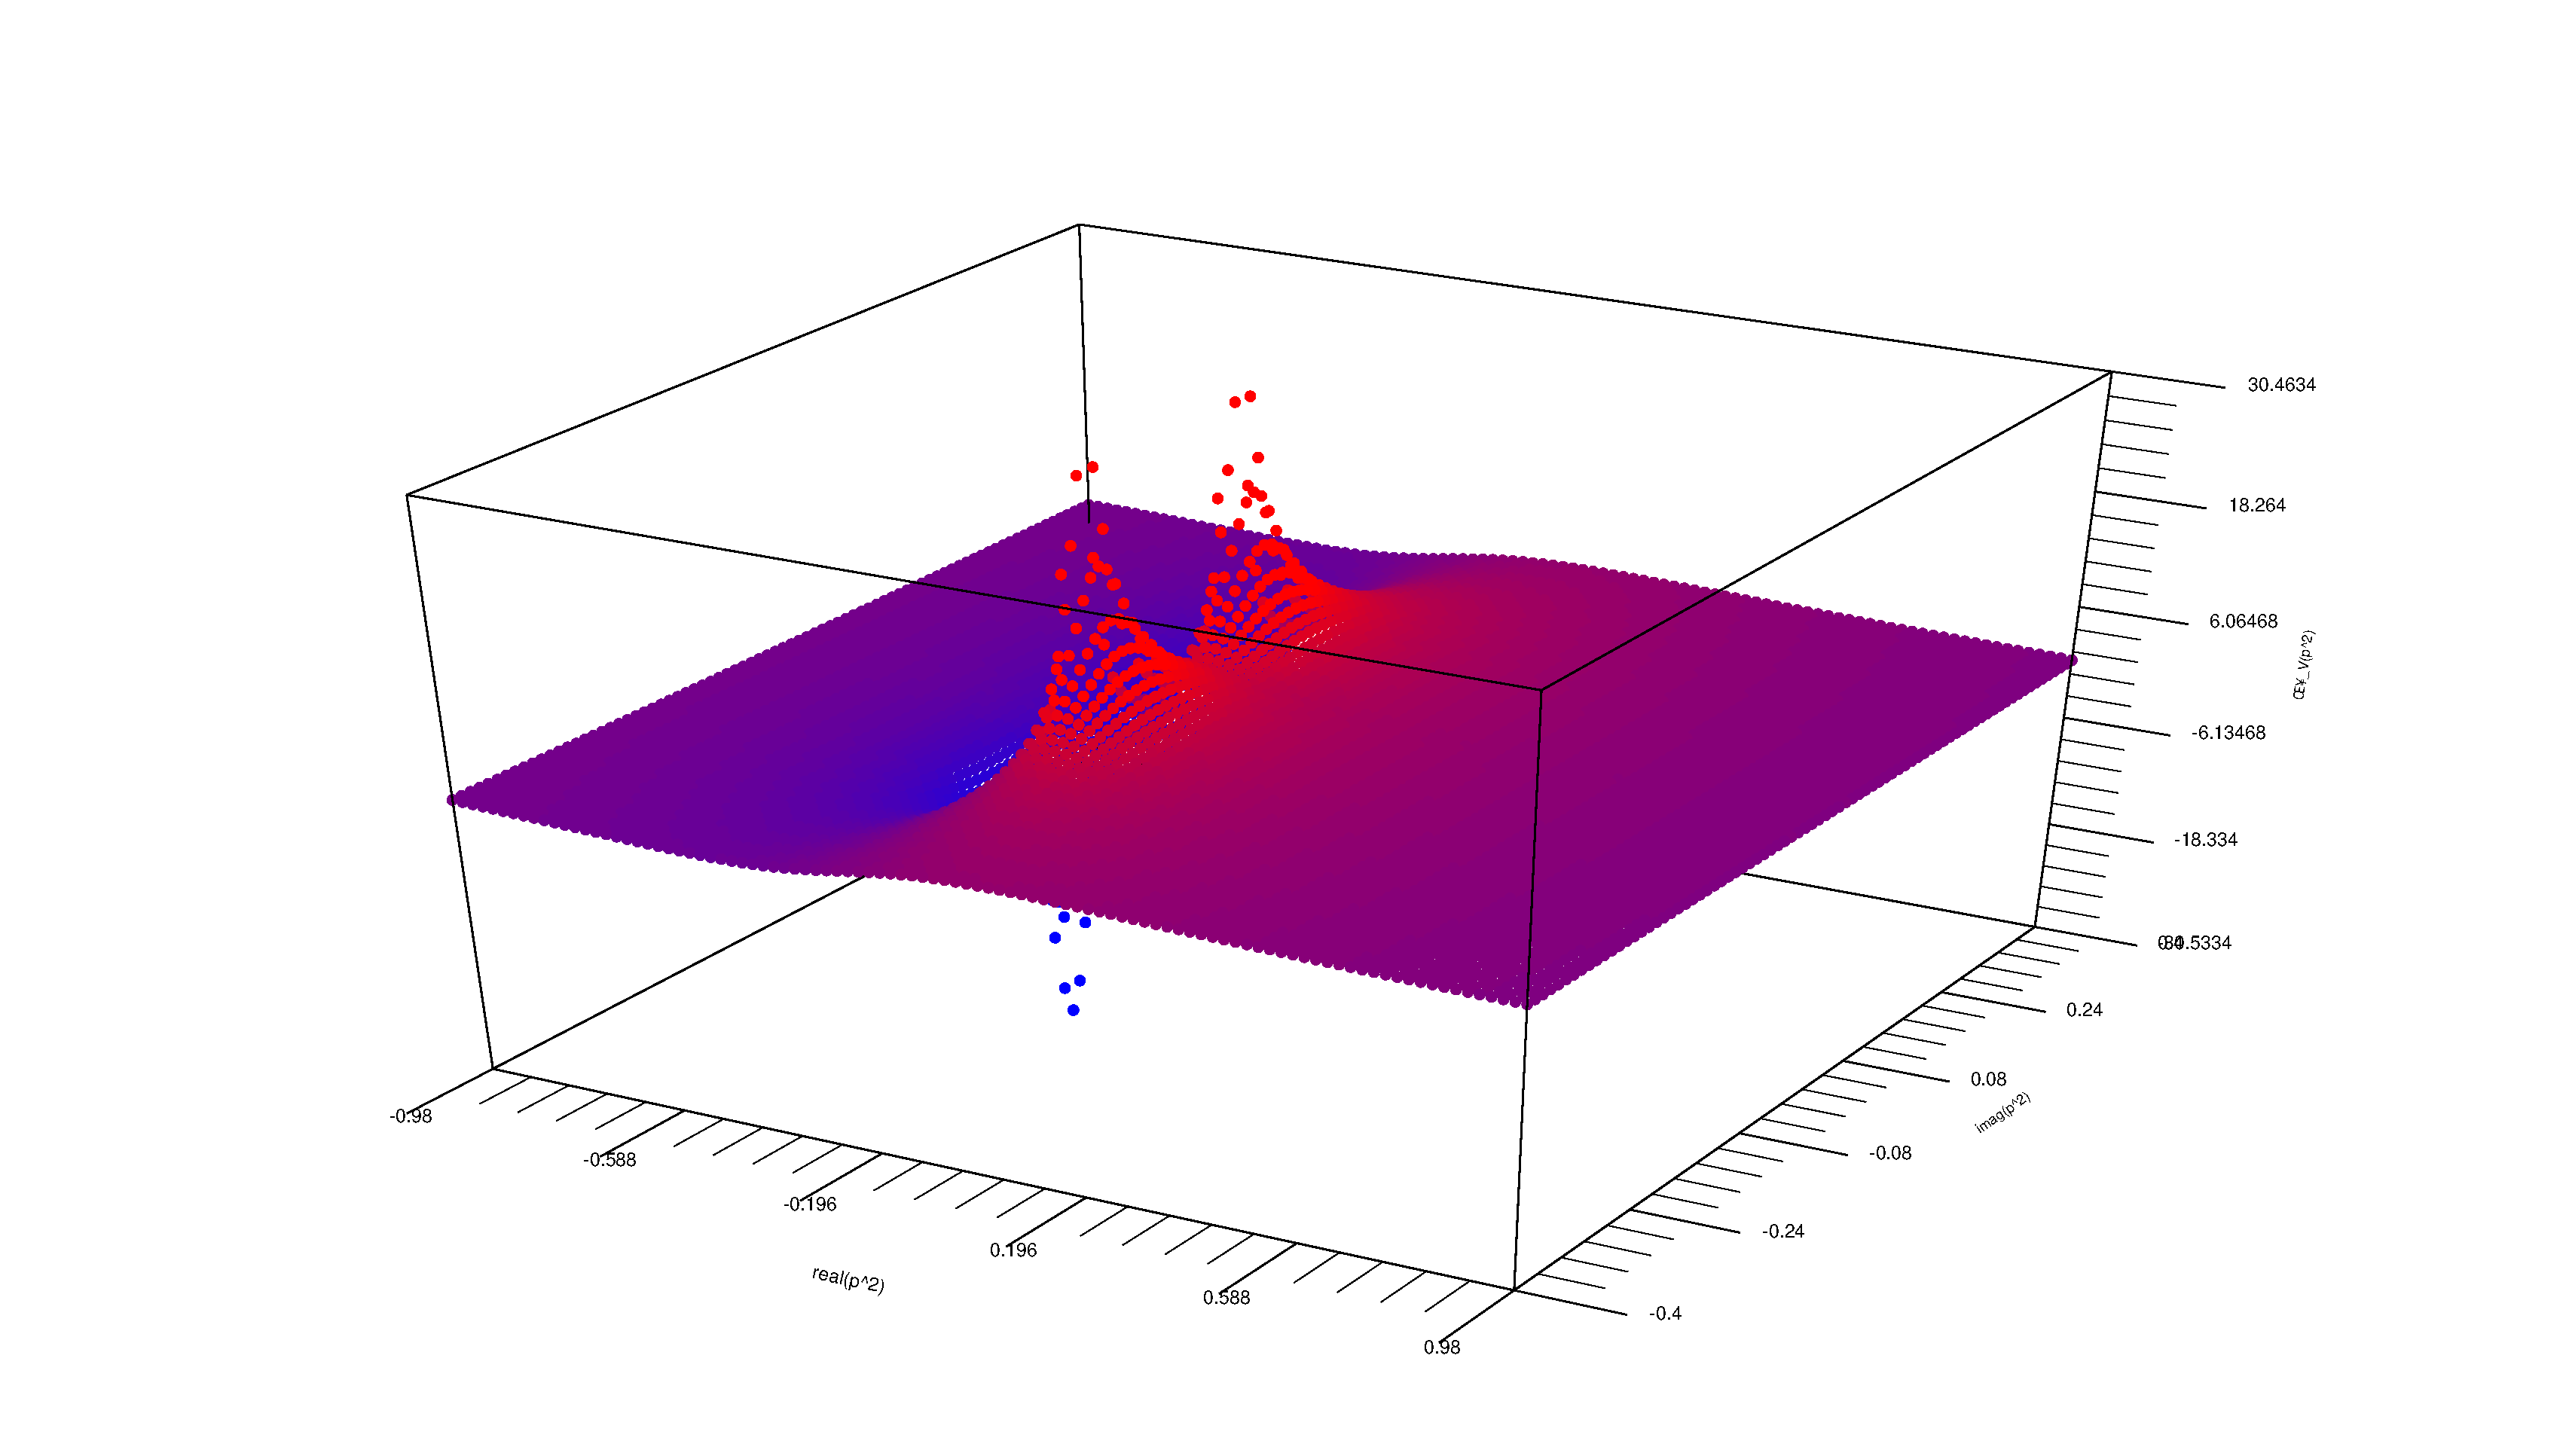
\includegraphics[width=1.1\textwidth]{figures/sigma_poles}
 \end{center}
 \caption{\footnotesize Analytic continuation of quark dressing $\sigma_V$. }\label{fig:sigma_poles} 
\end{figure}

Recall, the inverse quark propagator is given in the form:
\beqa
	S(p) =i \sigma_v(p^2) \pslash + \sigma_s(p^2)\;,
\eeqa
whether the inverse one:
\beqa
	S^{-1}(p)=-i A(p^2)\pslash + B(p^2)
\eeqa
	As we can see from Fig. and Fig. the quark propagator has two poles, that come from the common denominator in $\sigma_v$ and $\sigma_s$ functions:
\beqa
	\frac{1}{A^2 p^2 + B^2}
\eeqa
Note however, these poles are not corresponding to asymptotic state, since they are not lying on real $P^2$ axis. Also it was shown in \cite{Fischer:2008sp} that the inclusion of the pion cloud effect does not change the non-analytic structure of the quark, as it was required from Gribov's supercriticality picture of quark confinement.
\begin{figure}[H]
\tiny
 \begin{center}
  \includegraphics[width=0.95\textwidth]{figures/shift_momenta}
 \end{center}
 \caption{\footnotesize Shifting momenta routing. }\label{fig:shift_momenta} 
\end{figure}
	In order to be able to perform similar continuation for the DSE with pion cloud effect included we need to change momenta routing in a such way, that integration real $k$-momentum would flow through gluon and pion propagators and complex $q=p-k$ would go though quark propagator. This is diagrammatically given in Fig. \ref{fig:shift_momenta}. This allows us to solve two problems in the same time: firstly, use Maris-Tandy model on real axis as it is meant to be used; secondly, do not hit a pole in pion propagator $D_\pi(k^2)=\frac{1}{k^2+M^2_\pi}$. However it requires more sophisticated numerical approach in order to solve quark DSE - so-called "Grid-to-Contour" iteration, which is described in Appendix \ref{app:numerics}. \\ 
	
	At this point we considered a key piece in whole DSE/BSE calculation framework: the quark \DS equations. We studied its various truncations and physical meaning behind them. We obtained the solutions associated with quark DSE in rainbow-ladder and pion cloud truncations, observed the dynamical chiral symmetry breaking and continued these solutions into time-like region for the further use in meson \BS equations. 